\documentclass[14pt]{extarticle}

\DeclareMathSizes{14}{14}{15}{12}

\renewcommand{\normalsize}{\fontsize{14}{16}\selectfont}


% Language setting
% Replace `english' with e.g. `spanish' to change the document language
\usepackage[english]{babel}
\usepackage{graphicx}
\graphicspath{ {./images/} }
% Set page size and margins
% Replace `letterpaper' with `a4paper' for UK/EU standard size

\usepackage[letterpaper,top=2cm,bottom=2cm,left=3cm,right=3cm,marginparwidth=1.75cm]{geometry}

% Useful packages
\usepackage{amsmath}
\usepackage{graphicx}
\usepackage[colorlinks=true, allcolors=blue]{hyperref}

\title{TP3 Automatique - Sami BOUFASSA}

\begin{document}
\maketitle


Question 1 :

\begin{figure}[tbh]
    \vspace{0.1cm}
        \centering
        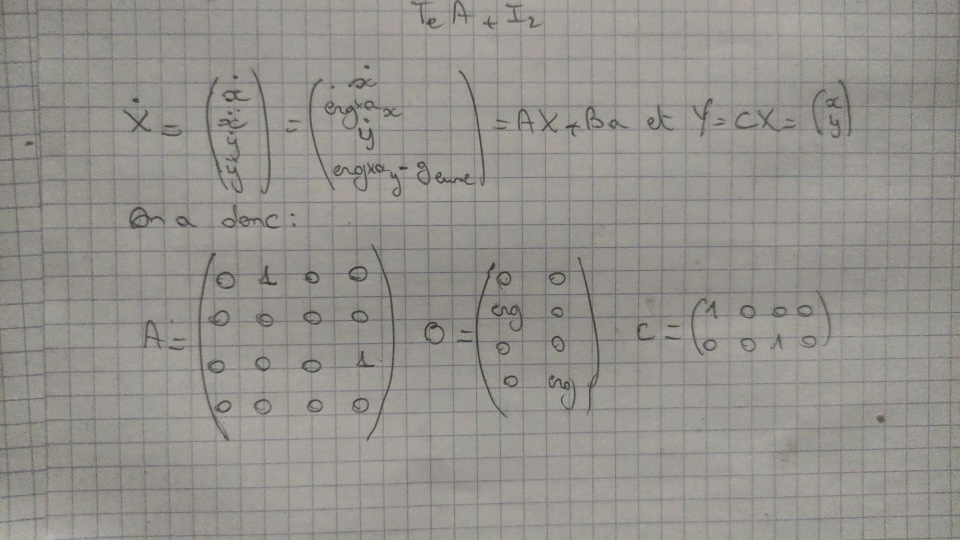
\includegraphics[width=\columnwidth]{"images/q1.jpg"}
    
    \end{figure}



Question 2 :

\begin{itemize}
    \item Le vecteur d'etat X contient toutes les variables necessaires pour decrire le mouvement du Lunar Lander autrement dit les positions (x,y) et les vitesses ($\dot x$, $\dot y$). 
    \item La derivee du vecteur d'etat est bien une combinaison lineaire des etats et des entrees $a_x$ et $a_y$ des moteurs du Lunar Lander.
    \item La sortie Y est une combinaison lineaire des etats du vecteur d'etat (et des entrees). 
    \item Toutes les lignes de la derivee du vecteur d'etat sont lineairement independantes. 
\end{itemize}


Questions 3 et 4 :
\begin{figure}[tbh]
    \vspace{0.1cm}
        \centering
        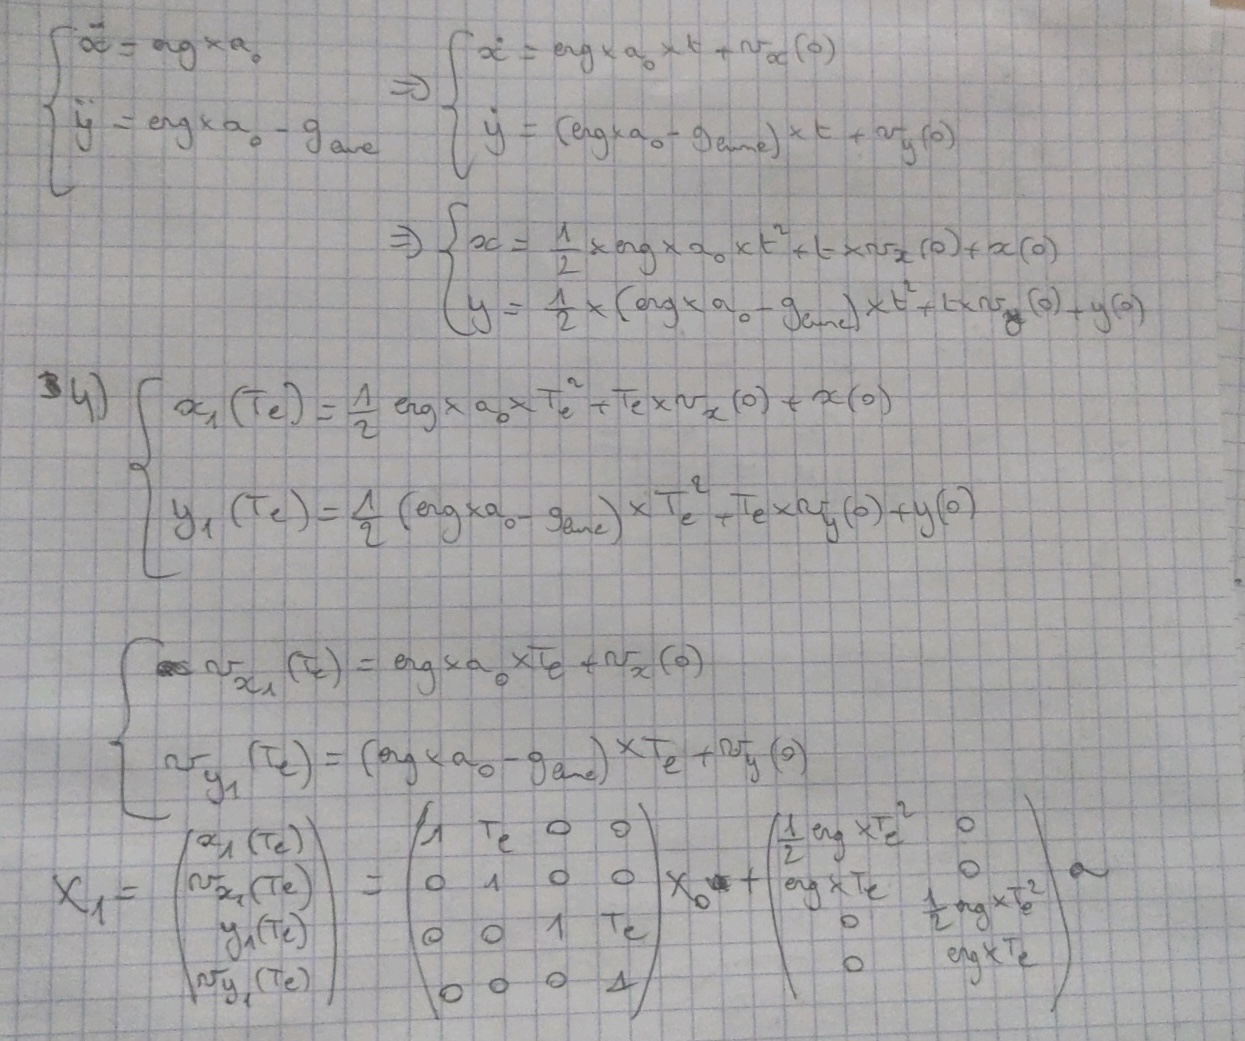
\includegraphics[width=\columnwidth]{"images/q3_q4.jpg"}
    
    \end{figure}





\break 
Question 5 : 

\begin{figure}[tbh]
    \vspace{0.1cm}
        \centering
        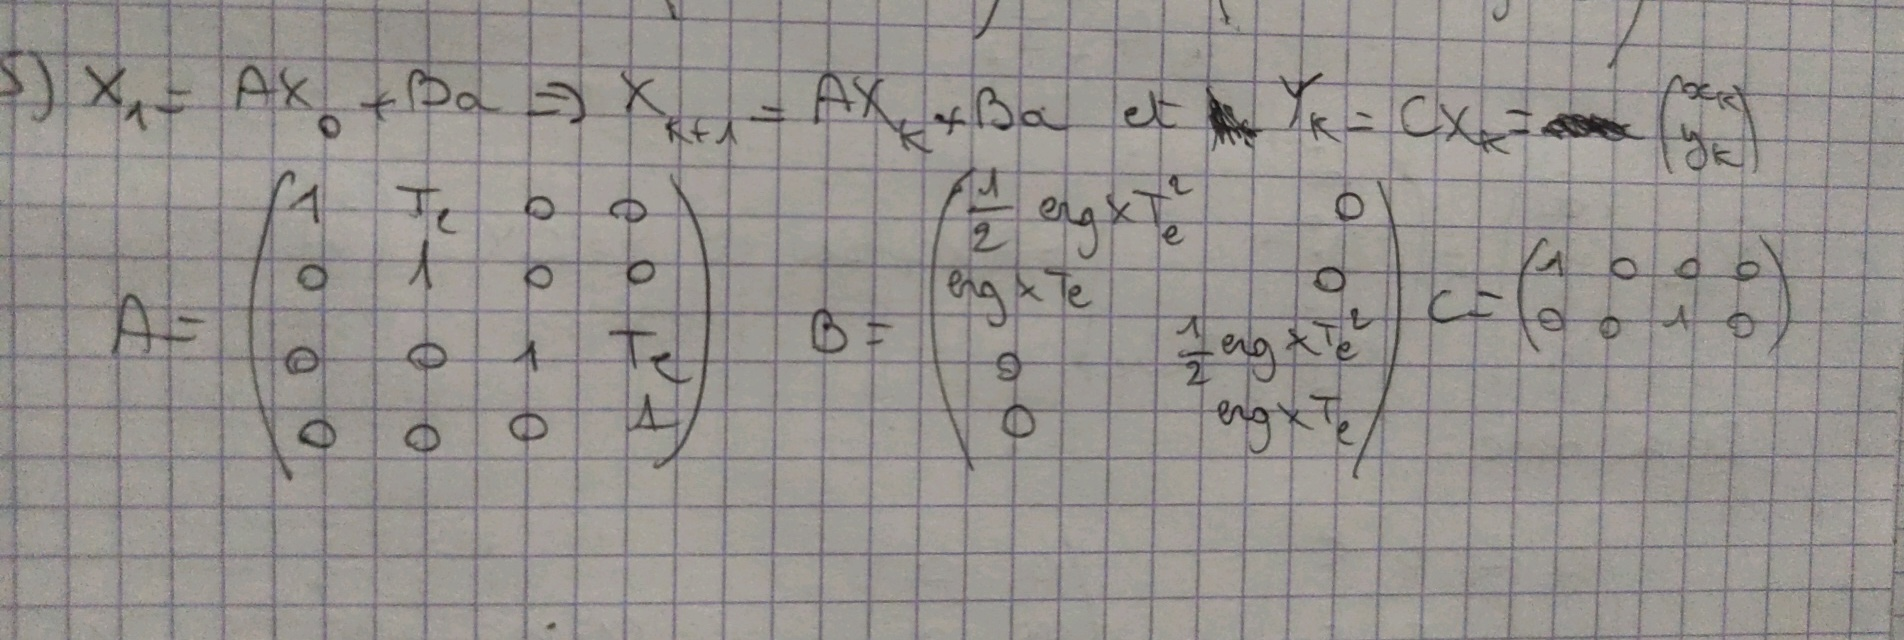
\includegraphics[width=\columnwidth]{"images/q5.jpg"}
    
    \end{figure}

\vspace{0.5cm}

Question 6 :

    Les équations gouvernant le mouvement en x ne dépendent que des variables associées à x (position et vitesse en x), tandis que celles en y ne sont fonction que des variables liées à y (position et vitesse en y).

\break
Questions 7 et 8 :
\newline 

\begin{figure} [tbh]
\vspace{0.1cm}
\centering
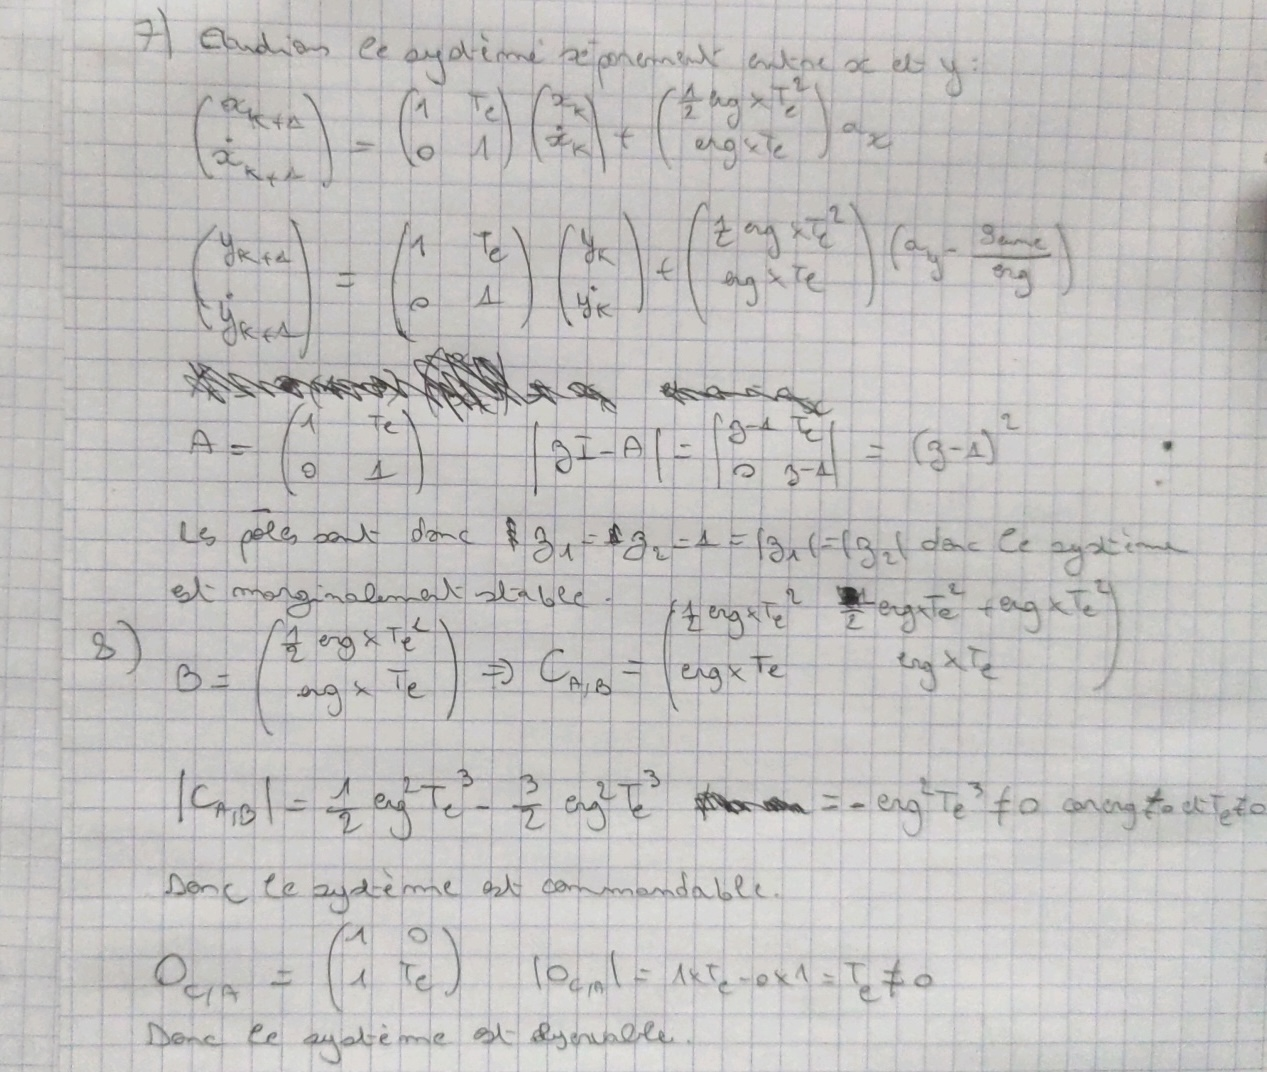
\includegraphics[width=\columnwidth]{"images/q7_q8.jpg"}
        
\end{figure}

\break 

Question 10 : 

a) Le Lunar Lander se déplace sous l'effet de la gravité lune sans propulsion, avec une vitesse initiale non nulle. L'équation de sa trajectoire est décrite par :
\[y = \frac{-1}{2}g_{\text{lune}}(\frac{x}{2} -1)^2 + 100\]
Il agit comme un projectile en chute libre, où la gravité gouverne son mouvement sans toute autre force extérieure, à l'exception de son mouvement initial.
\begin{figure} [tbh]
    \vspace{0.1cm}
        \centering
        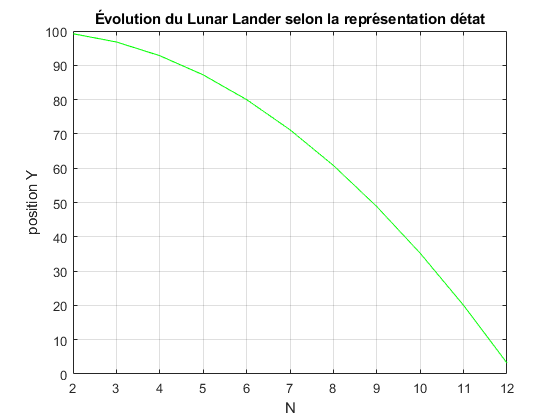
\includegraphics[width=\columnwidth]{"images/q10_1.png"}
    
    \end{figure}

b) La résultante des forces selon l'axe y est nulle, c'est-à-dire que la force de poussée $erga_y$ équilibre exactement la force gravitationnelle de la lune, ce qui donne :
\[erga_y - g_{\text{lune}} = 0\]

L'équation de sa trajectoire est alors décrite par $x =  1000$ et $y = 100$.

Dans ce cas, le Lunar Lander se déplace uniquement le long de l'axe x, avec une position constante sur l'axe y à y=100.
\begin{figure} [tbh]
    \vspace{0.1cm}
        \centering
        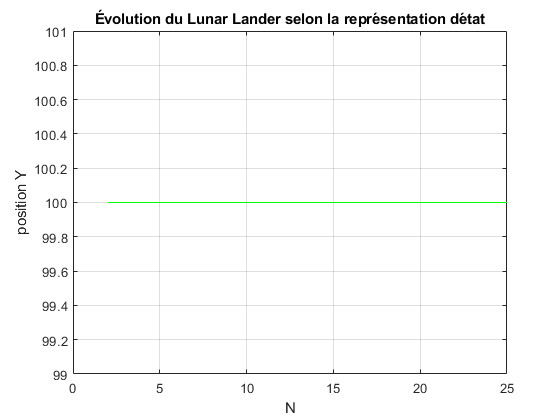
\includegraphics[width=\columnwidth]{"images/q10_2.png"}
    
\end{figure}


\begin{figure} [tbh]
    \vspace{0.1cm}
        \centering
        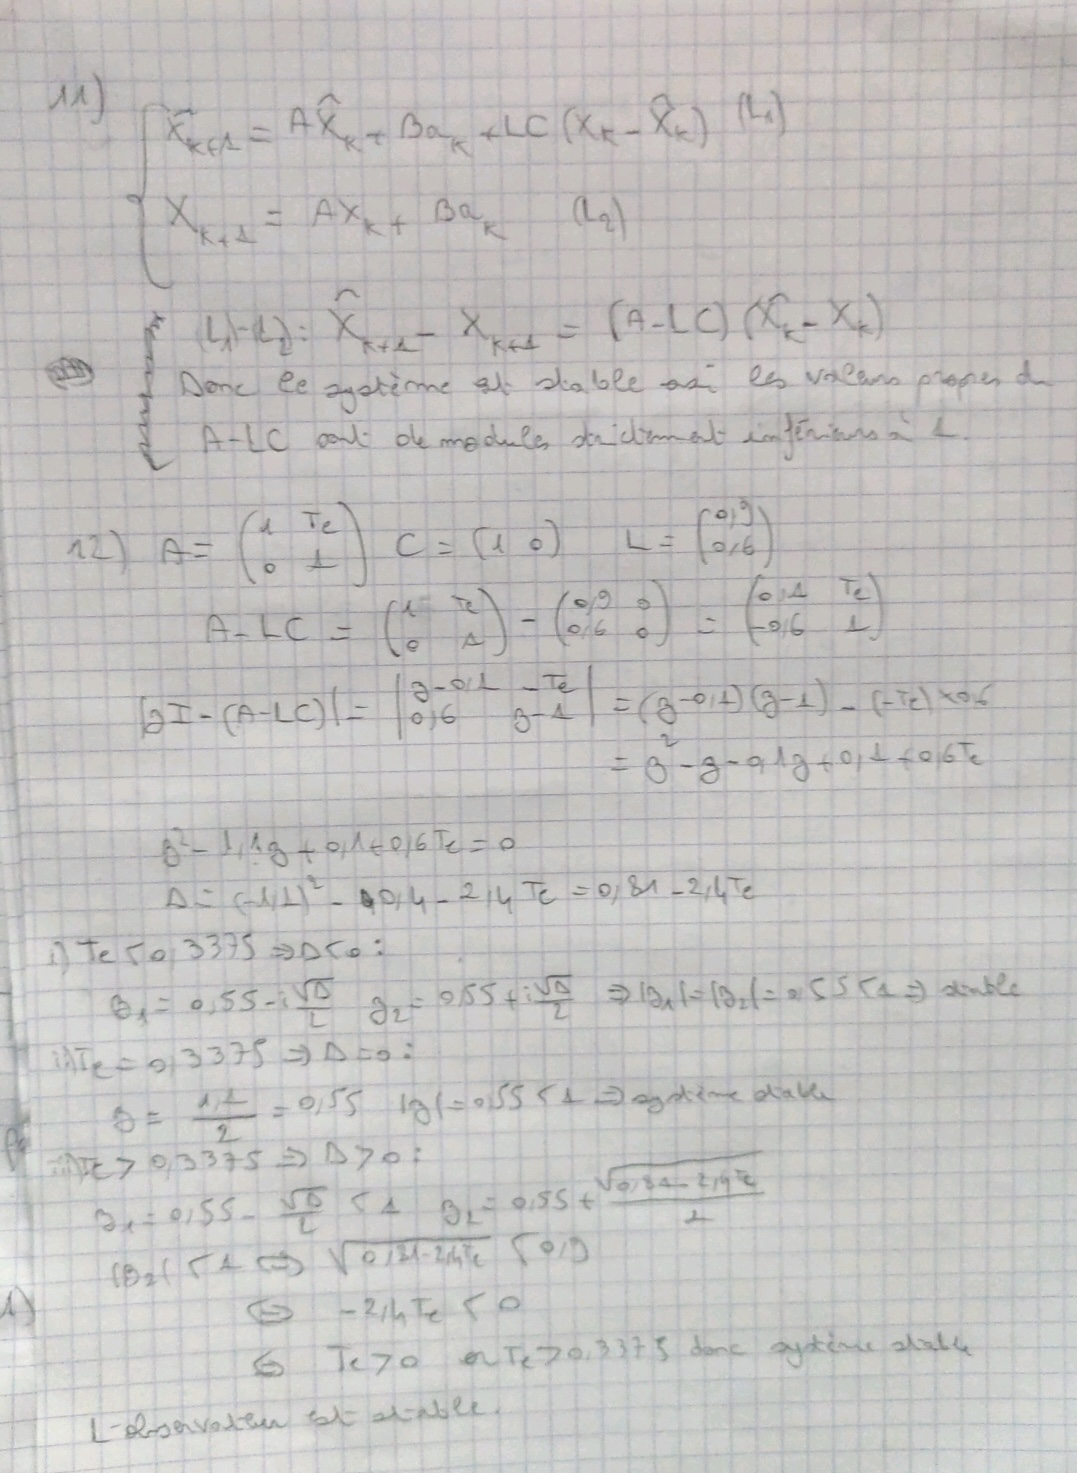
\includegraphics[width=\columnwidth]{"images/q11_q12.jpg"}
    
    \end{figure}

\break

Question 13 :

\break 
a) 

\begin{figure} [tbh]
    \vspace{0.1cm}
        \centering
        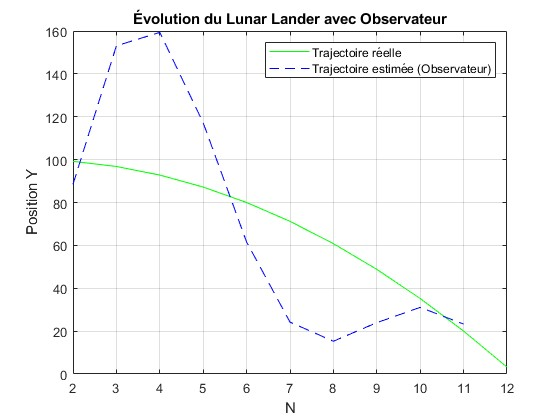
\includegraphics[width=\columnwidth]{"images/q13_1.jpg"}
    
    \end{figure}

b) 
\begin{figure} [tbh]
    \vspace{0.1cm}
        \centering
        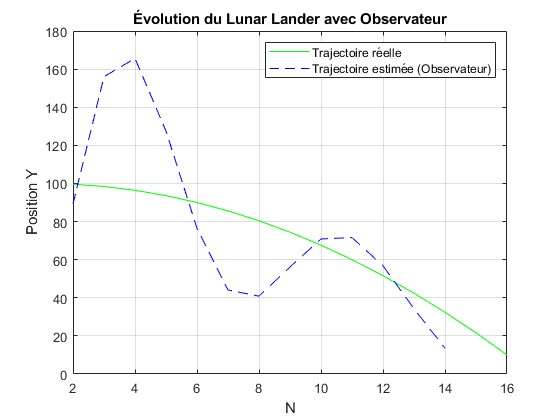
\includegraphics[width=\columnwidth]{"images/q13_2.jpg"}
    
    \end{figure}
Question 14 : 
    Dans les 2 cas, on remarque un dépassement de la position estimée par rapport à la position réelle au début du tracé puis la position estimée converge finalement vers la position réelle.
Les graphes sont en accord avec le constat sur la stabilité de l'observateur trouvée en Question 12. L'observateur remplit bien
son rôle.
\end{document}
	
